\newcommand{\cnt}{c}
\newcommand{\meas}{\epsilon}
\newcommand{\dt}{\Delta t}
\newcommand{\dtm}{\dt_{\meas}}
\newcommand{\dtc}{\dt_{\cnt}}
\newcommand{\Ncm}{{n_{\sfrac{\cnt}{\meas}}}}
\newcommand{\Nmnd}{{n_{\sfrac{\meas}{zc}}}}
\newcommand{\Nnd}{{n_{zc}}}
\newcommand{\Nm}{{n_{\meas}}}
\newcommand{\Ncnt}{{n_{\cnt}}}
\newcommand{\LTb}{\tau_b}
\newcommand{\LTd}{\tau_d}
\newcommand{\lamb}{\lambda_b}
\newcommand{\lamd}{\lambda_d}

\DeclareDocumentCommand{\mupp}{s}{\mu'_\phi\IfBooleanTF{#1}{}{(t_i)}}
\DeclareDocumentCommand{\mudpp}{s}{\mu''_{\phi^2}\IfBooleanTF{#1}{}{(t_i)}}
\newcommand{\pars}{\boldsymbol{\theta}}
\DeclareDocumentCommand{\XpctO}{m}{\Xpct{#1}[\pars_0]}
\DeclareDocumentCommand{\var}{O{}mo}{\mathrm{var}_{#1}\bkt*{#2\IfValueT{#3}{\vert~ #3}}}
\DeclareDocumentCommand{\Fisher}{O{}D(){\pars_0}}{I_{#1}(#2)}
\newcommand{\y}{\mathbf{y}}

\usepgfplotslibrary{fillbetween}

\chapter{Статистическое моделирование}\label{Apx:Stats}
В этой главе мы рассматриваем стандартную ошибку оценки частоты прецессии спина, 
в эксперименте по поиску ЭДМ дейтрона в накопительном кольце. 
Основное рассмотрение начинается с раздела~\ref{Apx:Stats:Detector_counting_rate}; 
раздел~\ref{Apx:Stats:Prelim} предоставляет обоснование некоторым используемым понятиям 
(таким как информация Фишера выборки, информативность точки), но может быть пропущен.

Частота прецессии спина определяется путём фитирования данных поляриметрии синусоидальной функцией
 ${f(t) = a\cdot\sin(\w\cdot t + \delta)}$ с постоянными параметрами $(a,\w,\delta)$. 
 Данные о поляризации получают при рассеянии пучка на углеродной мишени. 
 Двумя важными обстоятельствами поляриметрии являются:
\begin{enumerate*}[(1)]
	\item уменьшение числа частиц в пучке при каждом измерении поляризации, и
	\item деполяризация.
\end{enumerate*}

В связи с первым обстоятельством возникает желание использовать каждое измерение поляризации 
максимально эффективно. В выборке измеренний сигнала, максимальной информативностью обладают точки,
измеренные в моменты, когда сигнал имел наибольшую скорость изменения 
(см. раздел~\ref{Apx:Stats:Prelim} ниже). По этой причине возникла идея измерять поляризацию пучка 
только в моменты пересечения ею нуля (модулированная схема измерения): 
таким образом увеличивается время жизни пучка, а потеря частиц происходит наиболее выгодным образом. 

При этом необходимо отметить, что анализирующая способность детектора как раз максимальна в экстремумах, 
и стремится к нулю в узлах сигнала. Это ограничивает возможность увеличения эффективности выборки
модулированной схемой: наиболее ценные для нас измерения поляризации имеют наименьшую точность, 
а наименее ценные --- максимальную. В связи с этим, мы пришли к выводу о нецелесообразности использования
модулированной схеме выборки.

Также, это влияет и на гетероскедастичность данных: в  проведённой нами симуляции 
мы использовали непериодическую модель роста ошибки стандартного отклонения 
измерения поляризации из~\cite[стр.~18]{Eversmann:Thesis}, в то время как 
колебания анализирующей способности детектора вводят периодическую зависимость от времени.

Фактор деполяризации в свою очередь ограничивает наши возможности по продлению времени жизни пучка, 
а следовательно накладывает ограничения и на длительность измерительного цикла, 
возможную точность единичной оценки частоты спин-прецессии, 
и длительность полного времени измерения ЭДМ.

В следующих разделах мы рассмотрим модель временн\'{о}й зависимости частоты событий на детекторе, 
введём понятие асимметрии сечения взаимодействия, и определим адекватную, ввиду деполяризации,
длительность измерительного цикла. Также, мы промоделируем статистическую обработку данных, и 
попытаемся определить потенциал применения модулированной схемы измерения поляризации.

\section{Предварительный анализ}\label{Apx:Stats:Prelim}

Вероятность наблюдения величины ${y_i = y(t_i)}$, при ожидании $\mu(t_i)$ и нормальном распределении ошибки:
\begin{align*}
f(y_i|\pars) &= \frac{1}{\sqrt{2\pi\nu}}\exp\bkt{-\frac12\frac{(y_i - \mu(t_i))^2}{\nu}}, \\
\pars 		  &= (\nu,\w,\phi),\\
\mu(t_i) 	  &= N_0\bkt{1 + P\sin(\w t_i + \phi)}.
\end{align*}

Вероятность наблюдения набора измерений $\y = (y_1,\dots, y_K)$, предполагая что они все происходят из одного и того же распределения, это произведение вероятностей, взятое как функция параметров:
\begin{align*}
\mathcal{L}(\pars|\y) &= \prod_i f(y_i|\pars);
\shortintertext{логарифм вероятности}
\ell(\pars|\y) &= -\frac{K}{2}\log2\pi - \frac{K}{2}\log\nu - \frac{1}{2\nu}\sum_i\epsilon_i^2,
~ \epsilon_i = y_i- \mu(t_i).
\end{align*}
Обычными предположениями на ошибку измерений являются равенство нулю её ожидания, и строгая экзогенность:
\[
\XpctO{\epsilon_i} = \XpctO{t_i\epsilon_i} = 0.
\]

В нашем случае, связь между производными ождидания:
\begin{align*}
\mu'_\phi	&= N_0P\cos(\w t + \phi), \\
\mu'_\w &= t\cdot\mu'_\phi, \epsilon'_\xi = -\mu'_\xi.
\end{align*}

%% Производные логарифма вероятности:
%% \begin{align*}
%% \ell'_\nu 		&= -\frac{K}{2\nu} + \frac{1}{2\nu^2}\sum_i\epsilon_i^2;  & \\
%% \ell'_\w 	&= \frac1\nu\sum_i\mupp t_i\epsilon_i;  & \\
%% \ell'_\phi		&= \frac1\nu \sum_i \mupp\epsilon_i; & \\
%% %
%% \ell''_{\nu^2}		&= \frac{K}{2\nu^2} - \frac{1}{\nu^3}\sum_i\epsilon_i^2, 
%% 	&-\XpctO{\ell''_{\nu^2}} = \frac{K}{2\nu^2} - \frac{1}{\nu^3}\sum_i\nu = \frac{K}{2\nu^2};\\
%% \ell''_{\nu\w}	&= -\frac{1}{\nu^2}\sum_i\mupp t_i\epsilon_i, 
%% 	&-\XpctO{\ell''_{\nu\w}} = \frac{1}{\nu^2}\sum_i\mupp\XpctO{t_i\epsilon_i} = 0;\\
%% \ell''_{\nu\phi}	&= -\frac{1}{\nu^2}\sum_i\mupp \epsilon_i, 
%% 	&-\XpctO{\ell''_{\nu\phi}} = \frac{1}{\nu^2}\sum_i\mupp\XpctO{\epsilon_i} = 0; \\
%% \ell''_{\phi^2}		&= \frac1\nu\sum_i\bkt{\mudpp \epsilon_i - \bkt{\mupp}^2}, 
%% 	&-\XpctO{\ell''_{\phi^2}} = \frac1\nu\sum_i\bkt{\bkt{\mupp}^2 - \mudpp\XpctO{\epsilon_i}} = \frac1\nu\sum_i\bkt{\mupp}^2;\\
%% \ell''_{\phi\w}	&= \frac1\nu\sum_i\bkt{\mudpp t_i\epsilon_i - \bkt{\mupp}^2t_i}, 
%% 	&-\XpctO{\ell''_{\phi\w}} = \frac1\nu\sum_i\bkt{t_i\bkt{\mupp}^2 - \mudpp\XpctO{t_i\epsilon_i}} = \frac1\nu\sum_i t_i\bkt{\mupp}^2;\\
%% \ell''_{\w^2}	&= \frac1\nu\sum_i\bkt{\mudpp t_i^2\epsilon_i - \bkt{\mupp t_i}^2},
%% 	& -\XpctO{\ell''_{\w^2}} = \frac1\nu\sum_i\bkt{\bkt{t_i\mupp}^2 - \mudpp\XpctO{t_i^2\epsilon_i}} = \frac1\nu\sum_i\bkt{t_i\mupp}^2.
%% \end{align*}

\subsection{Дисперсия оценки частоты}
После вычисления производных логарифма вероятности (и их ожиданий), получим матрицу Фишера: 
\[
\Fisher = \begin{pmatrix}
\sfrac{K}{2\nu} & 0 								& 0 \\
0 				& \sfrac1\nu\sum\bkt{t_i\mupp}^2	& \sfrac1\nu\sum t_i\bkt{\mupp}^2 \\
0				& \sfrac1\nu\sum t_i\bkt{\mupp}^2	&\sfrac1\nu\sum\bkt{\mupp}^2
\end{pmatrix}.
\]
Определитель матрицы
\newcommand{\STM}{\alpha}
\[
|\Fisher| = \frac{K}{2\nu^3}\underbrace{\bkt{\sum\bkt{t_i\mupp}^2\sum\bkt{\mupp}^2 - \bkt{\sum t_i\bkt{\mupp}^2}^2}}_{\STM}.
\]
Ковариационная матрица
\[
vcov = \begin{pmatrix}
\sfrac{2\nu}{K}& 0									& 0				\\
0				&\nu\frac{\sum\bkt{\mupp}^2}{\STM}		&\nu\frac{\sum t_i\bkt{\mupp}^2}{\STM}\\
0				&\nu\frac{\sum t_i\bkt{\mupp}^2}{\STM}	&\nu\frac{\sum\bkt{t_i\mupp}^2}{\STM}
\end{pmatrix}.
\]

Дисперсия оценки частоты
\begin{equation}\label{eq:Var1}
\var{\hat{\w}} = \nu\frac{\sum\bkt{\mupp}^2}{\sum\bkt{t_i\mupp}^2\sum\bkt{\mupp}^2 - \bkt{\sum t_i\bkt{\mupp}^2}^2}.
\end{equation}

\paragraph{Проверка.} Положим ${\mu(t_i) = \phi + \w t_i}$. 

В этом случае ${\mupp = 1}$, 
${\mu'_\w(t_i) = t_i = t_i\cdot\mupp}$, и определитель матрицы Фишера упрощается:
\begin{align*}
|\Fisher| &= \frac{K}{2\nu^4}\bkt{K\sum_i t_i^2 - \bkt{\sum t_i}^2} \\
&= \frac{K^3}{2\nu^4}\bkt{\frac1K\sum t_i^2 - \avg{t}^2} \\
&= \frac{K}{2\nu^4}\cdot\underbrace{K\sum\bkt{t_i - \avg{t}}^2}_{\STM},
\end{align*}
\newcommand{\SSX}{\sum\bkt{t_i - \avg{t}}^2}
а ковариационная матрица становится
\[
vcov = \begin{pmatrix}
2\sfrac{\nu^2}{K}& 0									& 0				\\
0				&\frac{\nu}{\SSX}		&\nu\frac{\sum t_i}{K\SSX}\\
0				&\nu\frac{\sum t_i}{K\SSX}	&\nu\frac{\sum t_i^2}{K\SSX}
\end{pmatrix},
\]
с хорошо известным выражением дисперсии оценки наклона прямой
\[
\var{\hat\w} = \frac{\nu}{\SSX}.
\]

Обозначим ${\bkt{\mupp}^2 = (N_0P)^2\cos^2(\w t_i + \phi) \equiv x_i}$. 
Уравнение~\eqref{eq:Var1} может быть записано в виде:
\begin{align}
\var{\hat\w} &= \frac{\nu}{\sum_j x_j \bkt{\sum_i t_i^2 \frac{x_i}{\sum_j x_j} - \bkt{\sum_i t_i \frac{x_i}{\sum_j x_j}}^2}} \notag\\
&= \frac{\nu}{\sum_j x_j \sum_i w_i\bkt{t_i - \avg{t}[w]}^2} \notag\\
&= \frac{\nu}{\sum_j x_j \cdot\var[w]{t}}. \label{eq:Var2}
\end{align}
Здесь вариация $\var[w]{t}$ характеризует разброс выборки по независимой координате, 
и минимально чувствительна к выбранным точкам измерения, влияющим на $x_i$. В свою очередь, 
фактор $\sum_jx_j$ характеризует полную информацию Фишера выборки. 

%% \newcommand{\M}{\underline{\mathrm{M}}}
%% \newcommand{\T}{\underline{\mathrm{T}}}
%% \newcommand{\diag}[1]{\mathcal{D}_{#1}}
%% \newcommand{\diagM}{\diag{\mu}}
%% В матричном виде, дисперсия оценки частоты может быть записана как
%% \begin{align*}
%%   \var{\hat\w} &= \frac{\nu}{\bkt{\T'\diagM^2\T} - \bkt{\T'\diagM\M}^2/\bkt{\M'\M}}, 
%%   \shortintertext{with}
%%   \T &= \bkt{t_0,\dots, t_{K-1}}', ~ \M = \bkt{\mupp*(t_0),\dots,\mupp*(t_{K-1})}', \\
%%   \diagM &= \begin{pmatrix}
%%     \mupp*(t_0) & 0				& \cdots & 0 \\
%%     0			& \mupp*(t_1)	& \cdots & 0 \\
%%     \vdots		& \cdots		&\ddots	 & \vdots \\
%%     0			& 0				&\cdots  & \mupp*(t_{K-1})
%%   \end{pmatrix}.
%% \end{align*}

\subsection{Модуляция выборки}
Запишем матрицу Фишера в виде суммы
\begin{equation}\label{eq:FisherSum}
\Fisher = \sum_i \Fisher[i]; 
~\Fisher[i] = \frac1\nu\begin{pmatrix}
\bkt{\sqrt2\cdot\mupp}^{-2} & 0 		& 0 \\
0		 & t_i^2 	& t_i \\
0		 &	t_i	    & 1
\end{pmatrix}\cdot\bkt{\mupp}^2.
\end{equation}

$\Fisher[i] = -\XpctO{\frac{\partial^2}{\partial\pars^2}\log f(y_i|\pars)\vert_{\pars=\pars_0}}$ будем интерпретировать как информацию о параметре, заложенную в измерение $y_i$.
\begin{figure}[h]
	\centering
	\subbottom[Информация Фишера точки зависит параболически от производной сигнала.]{%
		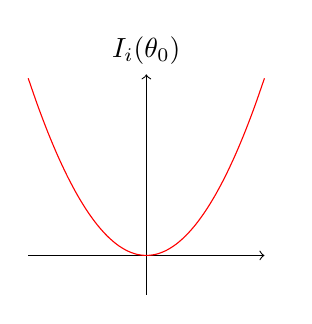
\begin{tikzpicture}
		\draw[->] (-1.5,0) -- (1.5,0) node[right] {$\mupp$};
		\draw[->] (0,-.5) -- (0, 2.3) node[above] {$I_i(\pars_0)$};
		\draw[scale=1,domain=-1.5:1.5,smooth,variable=\x,red] plot ({\x},{\x*\x});
		\end{tikzpicture}
	}
	\subbottom[Точки в заштрихованных областях более информативны.]{%
		\begin{tikzpicture}
		\begin{axis}[axis lines=center, xlabel=$t$, domain=-.5:2*pi, legend pos=outer north east]
		\addplot[color=blue, name path=signal, domain=-.1:2*pi,samples=50] {sin(deg(x))}; \addlegendentry{сигнал}
		\addplot[color=red, samples=50] {cos(deg(x))^2}; \addlegendentry{$\bkt{\mupp}^2$}
		\addplot[mark=none,dashed, domain=0:2*pi]{.5};
		\draw[dashed] (axis cs:.785,0) -- (axis cs:.785,{sin(deg(.785))});
		\draw[dashed] (axis cs:2.36,0) -- (axis cs:2.36,{sin(deg(2.36))});
		\draw[dashed] (axis cs:3.93,0) -- (axis cs:3.93,{sin(deg(3.93))});
		\draw[dashed] (axis cs:5.5,0) -- (axis cs:5.5,{sin(deg(5.5))});
		\path[name path=axis] (axis cs:0,0) -- (axis cs:2*pi,0);
		\addplot[fill=blue, opacity=.05] fill between [of=signal and axis, soft clip={domain=0:.785}];
		\addplot[fill=blue, opacity=.05] fill between [of=signal and axis, soft clip={domain=2.36:3.93}];
		\addplot[fill=blue, opacity=.05] fill between [of=signal and axis, soft clip={domain=5.5:2*pi}];
		\end{axis}     
		\end{tikzpicture}
	}
	\caption{Зависимость информации Фишера измерения синусоидального сигнала от его производной.}
\end{figure}

Если дать каждой точке вес, пропорциональный её информации Фишера, т.е. $w_i = \cos^2(\w t_i + \phi)$, вес области с $\bkt{\mupp}^2 \geq\sfrac12$ больше чем у эквивалентной области с $\bkt{\mupp}^2 < \sfrac12$ на множитель
\begin{align*}
\int_{t_0}^{t_1}\cos^2(\w t + \phi)\rd t = \frac1\w\int_{\w t_0+\phi}^{\w t_1+\phi} \cos^2\theta\rd\theta = \frac{\Delta t}{2} + \frac{1}{2\w}\sin\w\Delta t\cos\w\Sigma t \approx 1.9.
\end{align*}

То есть, если бы все точки находились в заштрихованной области, выборка была бы информативнее примерно в два раза.~\footnote{Это не учитывая что в случае поляриметрии неопределённость измерений обратно пропорциональна информативности, как было уже сказано во введении к этому приложению.}

\section{Модель частоты событий на поляриметре}\label{Apx:Stats:Detector_counting_rate}
В наших рассуждениях мы предположили следующую простую модель
изменения количества событий на поляриметре как функции времени:
\begin{equation}\label{eq:DetCntRt}
N(t) = N_0(t)\cdot\bkt{1 + P\cdot e^{-\sfrac{t}{\LTd}}\cdot\sin(\w\cdot t + \phi)},
\end{equation}
где $N_0(t)$ частота событий, связанная с неполяризованным сечением,
$\LTd$ время жизни поляризации, связанное с декогеренцией.

Ток пучка, рассеиваемого на мишени может быть описан с помощью:
\[
I(t)= I_0\cdot e^{t/\LTb} = \nu N_0^b\cdot e^{t/\LTb},
\]
где $\LTb$ --- время жизни пучка, $N_0^b$ его начальное число частиц,
и $\nu$ частота оборота пучка в ускорителе. Обозначая вероятность того, 
что рассеянная частица полетит в сторону детектора $p$, ожидаемое число
частиц, детектируемых в течении времени измерения $\dtc$ может быть
записано как
\begin{align}
N_0(t) & = p\cdot\int_{-\dtc/2}^{+\dtc/2} I(t+\tau)\rd\tau \notag                    \\
& = p\cdot\frac{\nu N_0^b}{\lamb} e^{\lamb t}\cdot \bkt{e^{\lamb\sfrac{\dtc}{2}} - e^{-\lamb\sfrac{\dtc}{2}}} \notag \\
& \approx \underbrace{p\cdot\nu N_0^b e^{\lamb t}}_{\text{rate}~r(t)} \cdot\dtc.
\end{align}
Таким образом, получаем распределение Пуассона
\[
P_{N_0(t)}(\tilde{N}_0) = \frac{\bkt{r(t)\dtc}^{\tilde{N}_0}}{\tilde{N}_0!}\cdot e^{-r(t)\dtc},
\]
с дисперсией $\SD{\tilde{N}_0}^2(t) = N_0(t)$. %In the limit of large $N_0(t)$, one can use the Gaussian approximation.

Нас интересует ожидаине $N_0(t) = \Xpct{\tilde{N}_0(t)}$, и его
стандартное отклонение $\SD{N_0}(t)$. Обозначая время измерения одного
события $\dtm$, полное время измерений $\dtc$, и число событий за
измерение $\Ncm = \dtm/\dtc$, ожидание
\begin{equation*}
\Xpct{\tilde{N}_0(t)}_{\dtm} = \frac{1}{\Ncm}\sum_{i=1}^\Ncm \tilde{N}_0(t_i).
\end{equation*}
Поскольку это сумма случайных переменных, $N_0(t)$ имеет нормальное
распределение; тогда стандартное отклонение среднего % abuse of notation here (SD in place of SE) for aesthetic reasons
\begin{align*}
\SD{N_0}(t) & = \SD{\tilde{N}_0}(t)/\sqrt{\Ncm} = \sqrt{N_0(t)\frac{\dtc}{\dtm}}            \\
& \approx \sqrt{\frac{p\cdot\nu N_0^b}{\dtm}}\cdot\dtc \cdot\exp\bkt{\frac{\lamb}{2}\cdot t}.
\end{align*}
\newcommand{\Acoef}{\frac{1}{\sqrt{p\cdot\nu N_0^b}}}

Отметим, что относительная ошибка растёт со временем:
\begin{equation}\label{eq:MeasRelErr}
\frac{\SD{N_0}(t)}{N_0(t)} \approx \frac{A}{\sqrt{\dtm}}\cdot\exp\bkt{-\frac{\lamb}{2}t} = \frac{A}{\sqrt{\dtm}}\cdot\exp\bkt{\frac{t}{2\LTb}},~ A=\Acoef.
\end{equation}

\section{Асимметрия сечения}
\newcommand{\Asym}{\mathcal{A}}
В качестве меры поляризации пучка используют асимметрию частоты
событий детекторов.~\cite[стр.~17]{Eversmann:Thesis} Асимметрия сечения
взаимодействия --- это нормализованная разность числа событий (в
единицу времени) на
детекторах, расположенных по разные стороны от вакуумной камеры:
\begin{equation}\label{eq:AsymDef}
\Asym = \frac{N(\frac\pi2) - N(-\frac\pi2)}{N(\frac\pi2)+N(-\frac\pi2)}.
\end{equation}

В нижеследующей симуляции, мы профитировали данные функцией:
\begin{equation}\label{eq:xFOM}
\Asym(t) = \Asym(0)\cdot e^{\lamd\cdot t}\cdot\sin\bkt{\w\cdot t + \phi},
\end{equation}
в которой, помимо частоты, оценивались параметры $\Asym(0)$, $\lamd$, и $\phi$. 

В связи с уменьшением числа частиц в пучке, измерение асимметрии
сечения гетероскедастично. Из~\cite[стр.~18]{Eversmann:Thesis}, мы приняли
модель гетероскедастичности
\begin{equation}\label{eq:AsymHtsk}
\SD{\Asym}^2(t) \approx \frac{1}{2N_0(t)}.
\end{equation}

\section{Оценка эффективной длительности измерительного цикла}
\DeclareDocumentCommand{\stat}{s}{\IfBooleanTF{#1}{X_{tot}}{\frac{\SD{\meas}^2}{\SE{\hat\w}^2\cdot \var[w]{t}}}}

\newcommand{\dtnd}{\dt_{zc}}
\newcommand{\SNR}{\text{SNR}}

Предположим нормальное распределение ошибки измерений, с нулевым
ожиданием и дисперсией $\SD{\meas}^2$. Эстиматор максимального
правдоподобия дисперсии оценки частоты колебаний асимметрии сечения
взаимодействия $\Asym$ может быть выражен как
\begin{align}
\var{\hat\w} &= \frac{\SD{\meas}^2}{X_{tot}\cdot \var[w]{t}}, \label{eq:VarW}
\shortintertext{где}
X_{tot} &= \sum_{j=1}^{\Nm} x_j = \sum_{s=1}^{\Nnd}\sum_{j=1}^{\Nmnd} x_{js}, \notag\\
\var[w]{t} &= \sum_i w_i \bkt{t_i - \avg{t}[w]}^2,~ \avg{t}[w] = \sum_i w_i t_i, \notag\\
w_i &= \frac{x_i}{\sum_j x_j},~ x_i = (\Asym(0)\exp(\lamd t_i))^2\cos^2(\w t_i + \phi) = \bkt{\mupp}^2. \notag
\end{align}

В выражении выше, $X_{tot}$ есть полная информация Фишера выборки, и
$\var[w]{t}$ --- мера длительности его измерения. Сумма по $s$ Можно наблюдать, что
выбирая подходящие моменты времени для измерения, можно увеличить
фактор $X_{tot}$, поскольку он пропорционален сумме производных сигнала по времени. 
Если частота и фаза колебаний уже известны до
приемлемого уровня, можно попытаться ещё улучшить эффективность измерений,
применяя схему выборки в которой измерения происходят только моменты быстрого
изменения сигнала (модулированная выборка).

Оба фактора $\var[w]{t}$ и $X_{tot}$ ограничены конечным временем
жизни поляризации. Поскольку мы измеряем колебательный сигнал, можно выразить 
${\sum_{j=1}^{\Nmnd} x_{js} = \Nmnd\cdot x_{0s}}$, для некоторого среднего значения $x_{0s}$ 
в данном узле $s$ колебаний, где $\Nmnd$ -- количество измерений асимметрии в окрестности узле. 
Будем называть \emph{временем сжатия}\footnote{Поскольку, не изменяя количества измерений 
	за единицу времени, они все ``сжимаются'' вокруг узла сигнала.} (обозначение $\dtnd$) 
период времени вокруг узла сигнала, в течении которого производятся измерения. 
Значение суммы
$\sum_{j=1}^{\Nmnd} x_{js}$ спадает экспоненциально из-за
деполяризации, так что $x_{0s} = x_{01}\exp{(\lamd\cdot \frac{(s-1)\cdot\pi}{\w})}$. Тогда:
\begin{align}
X_{tot} & = \Nmnd\cdot x_{01} \cdot \frac{\exp{\bkt{\frac{\lamd\pi}{\w}\Nnd}}-1}{\exp{\bkt{\frac{\lamd\pi}{\w}}}-1} 
\equiv \Nmnd \cdot x_{01}\cdot g(\Nnd); \label{eq:FItot}\\
x_{01}  & = \frac{1}{\dtnd}\int_{-\dtnd/2}^{+\dtnd/2}\cos^2(\w\cdot t)\rd t = \frac12\cdot \bkt{1 + \frac{\sin\w\dtnd}{\w\dtnd}},                                    \label{eq:MeanFIZC}   \\
\Nmnd   & = \frac{\dtnd}{\dtm}. \label{eq:NumMeasNode}
\end{align}

Уравнение~\eqref{eq:FItot} может быть использовано чтобы оценить
пределы длительности эксперимента. В Таблице~\ref{tbl:FItot} мы
собрали: процент от предела информации
Фишера сэмпла, время (как фактор времени жизни поляризации) исчерпания этого
процента информации из сэмпла, и соответствующее этому времени
отношение сигнал-шум. Отношение сигнал-шум вычислено по формуле:
\begin{equation}\label{eq:TauRatioSNR}
\SNR = \frac{\Asym(0)\cdot e^{-\sfrac{t}{\LTd}}}{\SD{\Asym}(t)} 
\approx \sqrt{2\cdot p\cdot\nu N_0^b\cdot \dtc}\cdot \Asym(0)\cdot \exp\bkt*{-\frac{t}{\LTd}\cdot\bkt{1+\frac12\frac{\LTd}{\LTb}}},
\end{equation}
в которой, полагая $\SD{\Asym(0)}/\Asym(0) \approx 3\%$ (точность
измерения поляриметрии), коэффициент перед экспонентой равен 33.
\begin{table}[h]
	\centering
	\caption{Выбранная информация Фишера, длительность измерений,
		соответствующее отношение сигнал-шум.\label{tbl:FItot}}
	\begin{tabular}{rrr}
		\toprule
		Предел ИФ(\%) & длительность ($\times\LTd$) &  SNR \\ \midrule
		95 &                    3.0 &  0.4 \\
		90 &                    2.3 &  1.1 \\
		70 &                    1.2 &  5.5 \\
		50 &                    0.7 & 11.7 \\ \bottomrule
	\end{tabular}
\end{table}

Предполагая отсутствие деполяризации ($\lamd=0$) и однородную выборку
с частотой $1/\dt$, уравнение~\eqref{eq:VarW} может быть записано
через физические переменные как
\begin{align*}
\stat* &= \sum_{k=1}^K \Asym^2(0)\cos^2(\w t_k + \phi) = \frac12 \Asym^2(0)\cdot K, \\
\var[w]{t} &= \sum_{k=1}^K(k\dt - \avg{t}[w])^2\underbrace{w_k}_{1/K} \\
&\approx \frac{\dt^2}{12}K^2 = \frac{T^2}{12},
\intertext{и тогда}					
\var{\hat{\w}} &= \frac{24}{KT^2}\cdot\bkt{\frac{\SD{\meas}}{\Asym(0)}}^2.
\end{align*}

\section{Результаты моделирования}\label{sec:stats:simulation}
\newcommand{\vp}[2]{{#1}\cdot 10^{#2}}
Мы симулировали сбор данных двух детекторов с параметрами собранными в
Таблице~\ref{tbl:DetCntRtParam} на протяжении $T_{tot}=1 000$~сек,
выбираемыми равномерно по времени с частотой $f_s = 375$~Гц.

Данные параметры симуляции были выбраны исходя из следующих
соображений: число частиц в пучке порядка $10^{11}$; если мы хотим
сохранить время жизни пучка равным времени жизни поляризации, мы не
можем исчерпать более 75\% от его начального числа частиц; всего лишь
1\% всех рассеяний на мишени полезны для поляриметрии, так что
остаётся $\vp{7.5}{8}$ полезных рассеяний. Измерение частоты событий
$N_0(t)$ с точностью примерно 3\% требует приблизительно 2 000 событий
на детекторе, что ещё уменьшает число измерений до ${\vp{3.75}{5}=f_s\cdot T_{tot}}$. 
Ожидаемая длительность цикла 1000 секунд, отсюда $f_s = 375$~Гц. 

Относительная ошибка измерения частоты событий на детекторах отражена на
Рисунке~\ref{fig:LRDetErr}; асимметрия сечения, вычисленная в
соответствии с уравнением~\eqref{eq:AsymDef}, представлена на Рисунке~\ref{fig:Asym}.
Данные асимметрии фитируются нелинейной, гетероскедастичной моделью
заданной как
\[
\Asym(t) = \Asym(0)\cdot e^{\lamd\cdot t}\cdot\sin\bkt{\w\cdot t + \phi},
\]
с функцией дисперсии весов заданной
уравнением~\eqref{eq:AsymHtsk}. Результаты фитирования представлены в Таблице~\ref{tbl:FitRes}.
\begin{table}[h]
	\begin{minipage}[t]{.5\linewidth}
		\centering
		\caption{Параметры модели частоты событий детекторов\label{tbl:DetCntRtParam}}
		\begin{tabular}[t]{cccc}
			\toprule
			         & Левый    & Правый        &         \\ \midrule
			$\phi$   & $-\pi/2$ & $+\pi/2$      & рад     \\
			$\w$     &  \multicolumn{2}{c}{3}   & рад/сек \\
			$P$      & \multicolumn{2}{c}{0.4}  &         \\
			$\LTd$   & \multicolumn{2}{c}{721}  & сек     \\
			$\LTb$   & \multicolumn{2}{c}{721}  & сек     \\
			$N_0(0)$ & \multicolumn{2}{c}{6730} &         \\ \bottomrule
		\end{tabular}
	\end{minipage}%
	\begin{minipage}[t]{.5\linewidth}
		\centering
		\caption{Результаты фитирования\label{tbl:FitRes}}
		\begin{tabular}[t]{crrc}
			\toprule
			           & Оценка & Ст. Ошибка      & Единицы \\ \midrule
			$\Asym(0)$ & 0.400  & $\vp{9.03}{-5}$ &         \\
			$\lamd$    & -0.001 & $\vp{7.86}{-7}$ & 1/сек   \\
			$\w$       & 3.000  & $\vp{7.55}{-7}$ & рад/сек \\
			$\phi$     & -1.571 & $\vp{2.25}{-2}$ & рад     \\ \bottomrule
		\end{tabular}
	\end{minipage}
\end{table}

\begin{figure}[H]
	\centering
	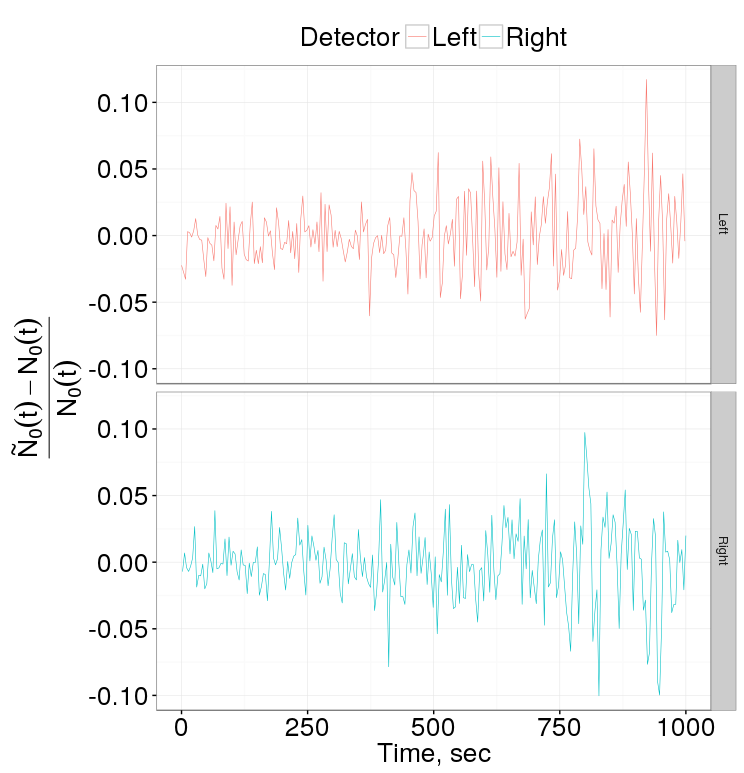
\includegraphics[width=.8\linewidth]{images/App_Stats/LR_detector_relErr}
	\caption{Относительная ошибка измерения частоты событий на правом и левом
		детекторах как функция времени.\label{fig:LRDetErr}}
\end{figure}

\begin{figure}[H]
	\centering
	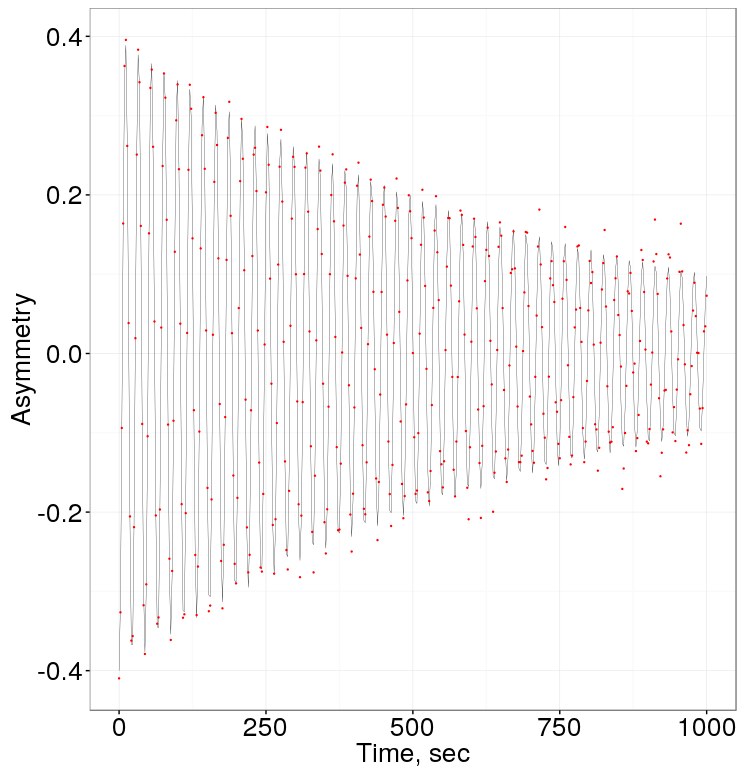
\includegraphics[width=.8\linewidth]{images/App_Stats/Asymmetry}
	\caption{Ожидание (чёрная линия) и измерения (красные точки)
		асимметрии сечения.\label{fig:Asym}}
\end{figure}

Если начальная оценка частоты, полученная из равномерной выборки, 
имеет стандартную ошибку порядка $10^{-6}$ рад/сек, симуляции
подтверждают, что при применении модулированной схемы выборки, 
стандартная ошибка оценки может быть улучшена до примерно $\vp{5.8}{-7}$ рад/сек, 
без учёта потери анализирующей способности детектора
при приближении вертикальной компоненты поляризации к нулю.

